\documentclass{utue} %uumi.cls required for Uni corporate design
\usepackage{listings}
\usepackage{url}
\usepackage{graphicx}
\usepackage{float}
\usepackage[margin=10pt,font=small,labelfont=bf]{caption}
\usepackage{multirow,booktabs,setspace,caption}
\usepackage{subfig}

\lstset{numbers=left, numberstyle=\tiny, numbersep=5pt, xleftmargin=10mm}

% Values for title generation
\title{Funfair: EEG-based game control}
\author{Robert Eisele \& Robert Geirhos}
\date{\today}

% Subtitle is optional. It represents what kind of work you did.
\subtitle{Praktikum Computergrafik WS2016/17}

\begin{document}

% You can place a teaser as follows. (Otherwise, just uncomment the following part)
\teaser{
    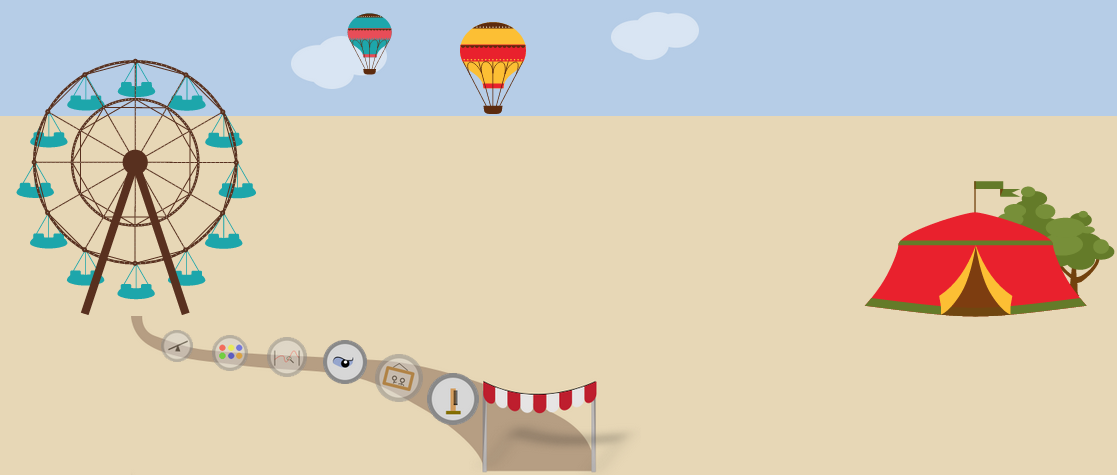
\includegraphics[width=\textwidth]{images/teaser_funfair.png}
    \caption{Screenshot of the funfair overview page.}
    \label{fig:teaser}
}     
%TODO idea: why not include a fancy animated video teaser here? That'd be beautiful...

% Creates title of document and additional title page.
\maketitle

\section*{Abstract}


Electroencephalography (EEG) is a technique for measuring brain activity. Although widely used in neuroscientific research, it has thus far only rarely been used for the purpose of computer game control. Here we show that a leightweight consumer EEG device, the Emotiv Insight\footnote{\url{https://www.emotiv.com/insight/}}, can be successfully used to play a broad range of simple yet challenging computer games. Furthermore, we demonstrate that rather than merely substituting a mouse or keyboard, an EEG device enables the development of a new type of games which go beyond traditional means of game control by enhancing human computer interaction. We specifically developed six browser games, all of which can be played by controlling one's mental activity. This could be be a starting point for a new, keyboard-free gaming experience.


% Give an overview over your project here. Give a glimpse insight in the problem and write why it is important to be solved. Write what you did to make your implementation better than the state of the art implementations.


\section{Introduction}

Traditionally, computer games are played with keyboard, mouse and more specialized input devices like a joystick, gamepad or a steering wheel. In order to improve gaming experience and making games as realistic as possible, much more sophisticated human computer interaction devices were developed, like virtual reality glasses and sensory gloves. Recently, affordable consumer EEG devices came to market, opening up the way for a completely new gaming experience: It might be possible to play a computer game without any visible action, simply by controlling some aspects of the own brain's activity. We aim to explore whether and if so, how well such a device, the Emotiv Insight, can be used to play computer games. The Emotiv Insight consists of enough sensors so that it might be possible to distinguish between several emotional levels and apply multiclass classification for sophisticated control mechanisms. If successfull, brain-controlled games could be used in a variety of settings: Not only as a new means of control for traditional games, and possibly for people unable to move their hands (e.g. due to a physical disablility after an accident or due to disease such as locked-in patients), but also as a starting point in the development of a different kind of games, namely games that cannot be played with traditional means of control because they require the gamer to be relaxed or focused - which would be difficult to realize with a keyboard! We here show that it is possible to use a customer EEG as the input device for six browser games.

Our report is organized as follows: After giving an overview over the technical aspects of our solution, we explain how the data were analyzed. We then explain our six games individually and discuss possible extensions.

\section{Description of the Solution}
We decided to develop browser games that go beyond a replacement of an ordinary keyboard or mouse. We therefore developed six small games, which can be subsumed under the topic of a funfair with several stalls, one per game. As the gamer succeeds in one game, playing the next one is unlocked as a reward, and the gamer moves closer to a big Ferris wheel (Fig. \ref{fig:teaser}) which is, upon successful completion of all six games, set into motion. We opted to create several small games (rather than one big monolithic game), as the focus would be shifted towards real game-development instead of focusing on bringing up simple yet working models that demonstrate different possibilities how brain-controlled gameplay can be achieved.

In order to get the best performance out of the sensor data, we first tried several ways of integrating the Emotiv sensor into an application. We started with the official Emotiv SDK, as it is available for several computer programming languages, like C\#, Java and Python. As the SDK turned out not to be sufficiently stable across different operating systems such as Linux and Mac OSX, we additionally looked at the Objective-C version (doing fine on OSX, but not under Linux). Since the features provided under the limiting licensing model as well as the limited data rate were not satisfying, we moved on and tried to reverse engineer the former Firefox extension, which was provided by Emotiv until December, 2016. As the official SDK as well as the Firefox extension did not provide the necessary data due to licensing problems and shut down of APIs, we eventually used the open source reverse engineered library Emokit by OpenYou\footnote{https://github.com/openyou}, which was initially developed to get data out of an Emotiv EPOC EEG headset, but flawlessly works with an Emotiv Insight headset as well.

Our software consists of a Python application, which forks a Tornado web-application server. This setup streams the sensor data from Emokit directly to the browser via websockets. On the browser side, the data is received asynchronously, both from the Emotiv data stream as well as from a Leap Motion sensor, which was used for one of the games to bring in another way of non-standard game interaction. The games themselves are organized in separate HTML files, which share one common JavaScript file. This JavaScript file handles the game-progress and implements a central animation loop which can be used by every individual game. Beyond that, it provides a small visual status bar, which indicates the current concentration level of the player.

\subsection{Sensor data analysis}
All data, if not stated otherwise, were analyzed using R \cite{RCoreTeam}. Our goal was to build several sensor data classifiers which, based on an analysis of the data, would be able to tell apart several menal states (\texttt{no\_action, action\_1, action\_2, ...}). In the process of building these classifiers, we faced two key challenges: Firstly, there was no prior mapping from the 16 sensors to a mental state - moreover, we did not know which sensor would correspond to which mental signal (like $ \alpha $ or $ \beta $ waves). Secondly, the sensor data - as is the case for almost any recorded data - seemed to be noisy. We therefore approached both challenges in a data-driven way: We recorded data for a variety of different actions and mental commands and carefully explored and visualized the sensor data recordings. As can be seen in Figure \ref{fig:sensor_values}, some commands such as \texttt{clench fist} were barely visible in the data, whereas other commands (e.g. \texttt{shake head, clench teeth}) produced considerably consistent spike-like patterns. We therefore decided to focus on the actions that seemed to be visually distinguishable in the data.

As most actions lasted for a very brief period of time, roughly 1-2 seconds, we buffered all sensor data individually with a sliding window of 2 seconds, which corresponds to 256 data points per sensor since the sampling frequency was 128 Hz, and took this sliding window as the basis for all further data analysis. We then implemented two different types of classification. The first one is a mapping based on a combination of several sensor values to a continuous value indicating the degree of relaxation (from tense, agitated to very relaxed and calm). It was achieved by taking into account the variance of the sum of all sensor data, which is based on the observation that a very tense state cannot be traced back to one particular sensor, but elicits high variance in several sensor recordings. The second type of classification, detecting discrete events, directly focuses on specific sensors: 
\texttt{Y} and \texttt{X} for \texttt{shake head} classification, \texttt{F3} for \texttt{nodding} and \texttt{O1} for the classification of \texttt{clench teeth}. It would have been possible to classify \texttt{squint eyes} as well, however the signals appeared to be hardly distinguishable from \texttt{clench teeth}, and needing to close one's eyes during gameplay was found to be rather annoying. This second type of classification was achieved through thresholding the windowed sample variance of a targeted sensor. As a result, we were able to classify one continuous mental state (\texttt{relaxation}) as well as four discrete events (\texttt{clench teeth, nodding, shake head, no\_action}).

\subsection{Gyro data analysis}

It turned out that Emokit was the perfect fit for our needs, as it gives raw measurements at a pretty high rate. Unfortunately, there is no documentation of what channel actually delivers what information. When the headset is moved around, a lot of channels dramatically change their values, which must be kept in mind for normal sensor analysis. 
%TODO low-pass filter (Robert E)

\subsection{Highstriker}
A highstriker is a classic game that can be found on most funfairs. We took the basic idea of striking with a hammer to achieve a score on a vertical bar and made a few adaptions to it. Rather than a using a virtual hammer, we mapped the current mental state to a score: the more relaxed one is, the better the score (and the friendlier the status indicator, ranging from \texttt{Burnout candidate} to \texttt{Master of Yoga}). As this game is, in our experience, both quite fun and very easy to play, we selected it to be the first game, enabling the user to get to know how he can control his mental activity to achieve a good score. This then prepares for more complex games such as the balancing game. So-called \textit{brain self-regulation} based on visual feedback has been successfully used in clinical settings, e.g. to teach psychopaths to control their aggression \cite{Konicar2015}. It would be interesting to see whether some of our games (the ones that can only be won when one learns how to calm down and relax quickly) could be used to train children suffering from ADHD (attention deficit hyperactivity disorder) in a fun way.

\subsection{Painter}
The core idea behind the painter game can be described as follows: Wouldn't it be fun to take a snapshot of yourself (using your computer's camera) and then having this image painted in a style that matches your mood? 

We achieved this by accessing the computer's camera through the browser, sending the plain image to the backend which forwards it, along with a style inferred from the current mood, to the Turbo-Deepart website\footnote{\url{http://turbo.deepart.io/}} via the DeepArt API\footnote{\url{https://github.com/deepart-io/deepart-api}} to paint the image, which is then subsequently sent back to the game. DeepArt basically implements a neural network-based technique for painting an input image in the style of an arbitrary style image \cite{Gatys2016}. For an illustration of how the Lena image looks like when painted in four different styles, see Fig. \ref{fig:painter_styles}. We were able to contribute a commit to the DeepArt API (\texttt{rgeirhos}, commit \texttt{50f200f}, merged Dec 14, 2016), solving an early image retrieval issue.

As an additional feature, the painted image is not only shown but lies behind a veil first (low alpha value). One then needs to use either the mouse to hover over the image and reveal it piece by piece, or use a Leap Motion controller\footnote{\url{https://www.leapmotion.com/}} to do so. A Leap Motion device measures hand gestures and translates them into a 3D hand model on the screen. We mapped the position of the hand model to a certain position on the canvas, which enables the user to simulate holding a paint brush in his or her hands and paint the image with painting-like movements.

\begin{figure}
	\centering
	\subfloat{
\includegraphics[width=0.22\columnwidth]{images/lena_6.jpg}}\hspace{0.02\columnwidth}
	\subfloat{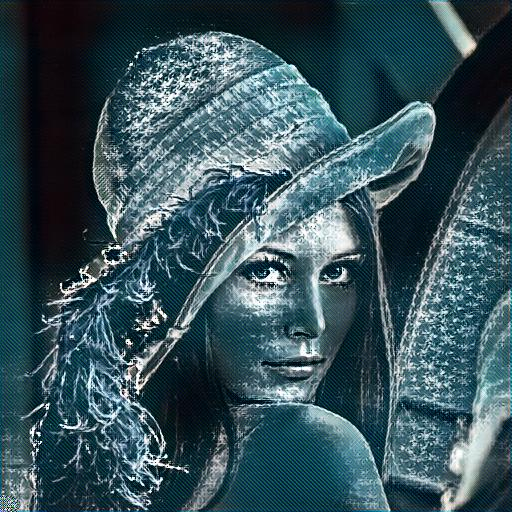
\includegraphics[width=0.22\columnwidth]{images/lena_24.jpg}}\hspace{0.02\columnwidth}
	\subfloat{
\includegraphics[width=0.22\columnwidth]{images/lena_26.jpg}}\hspace{0.02\columnwidth}
	\subfloat{
\includegraphics[width=0.22\columnwidth]{images/lena_21.jpg}}
	\caption{Four different style examples for the painter game. Images are sorted from a relaxed, calm style (left) to a more excited, agitated style (right).}
	\label{fig:painter_styles}
\end{figure}

\subsection{Magic Duel}


\begin{figure*}[t]
	\subfloat[Highstriker]{\label{ex0}
		
\includegraphics[width=0.25\textwidth]{images/highstriker.png}}\hfill
	\subfloat[Painter]{\label{ex1}
		
\includegraphics[width=0.25\textwidth]{images/painter.png}}\hfill
	\subfloat[Magic Duel]{\label{ex3}
		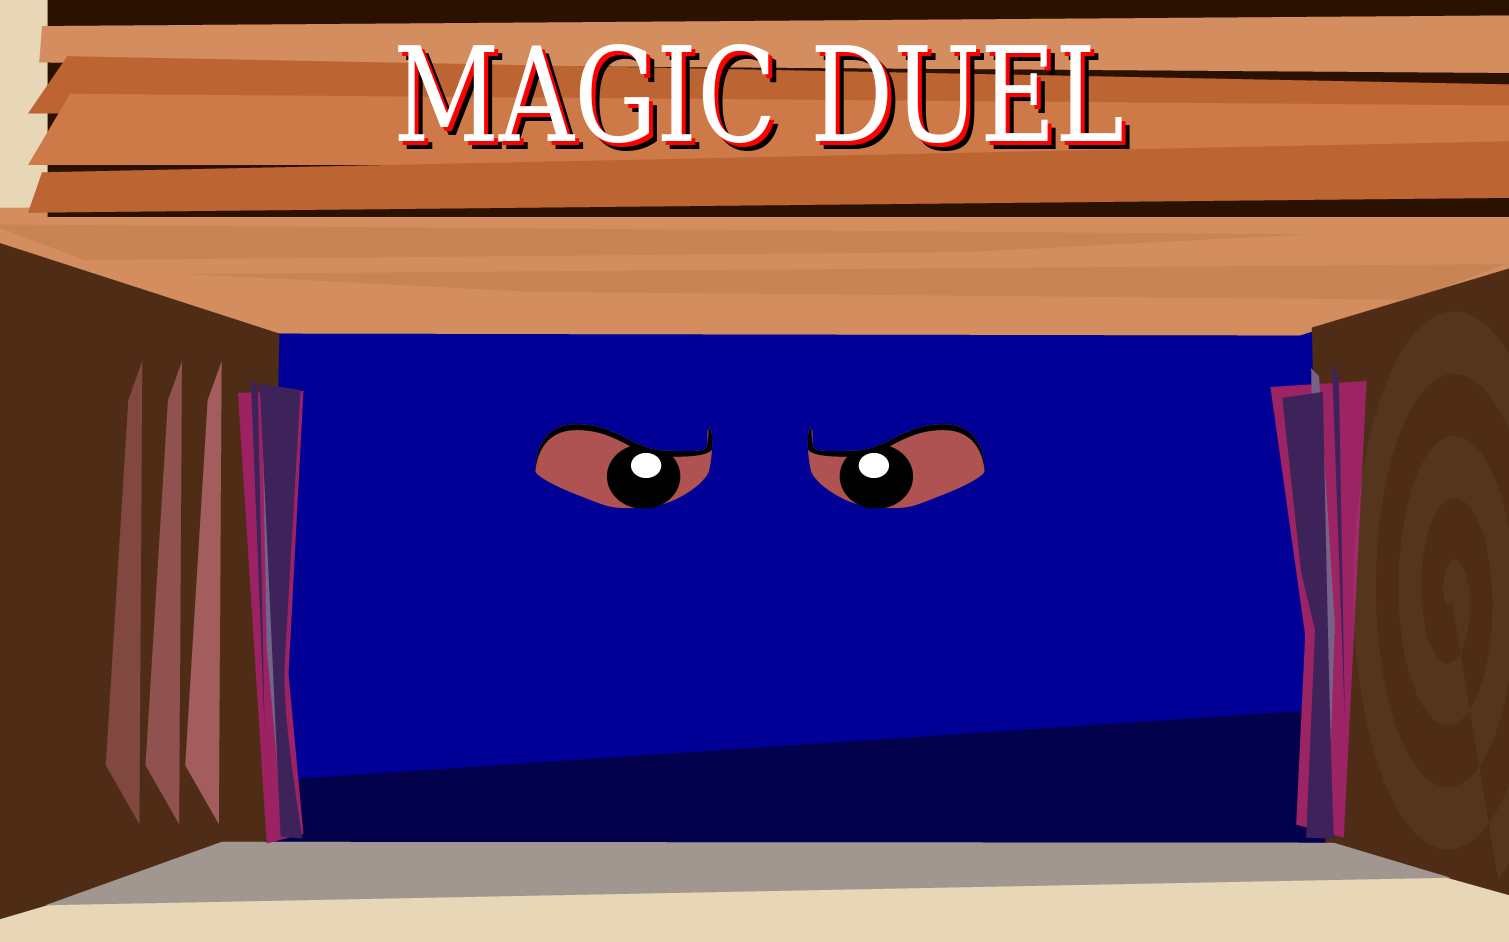
\includegraphics[width=0.25\textwidth]{images/magic.png}}\
	\subfloat[Wireloop]{\label{ex4}
		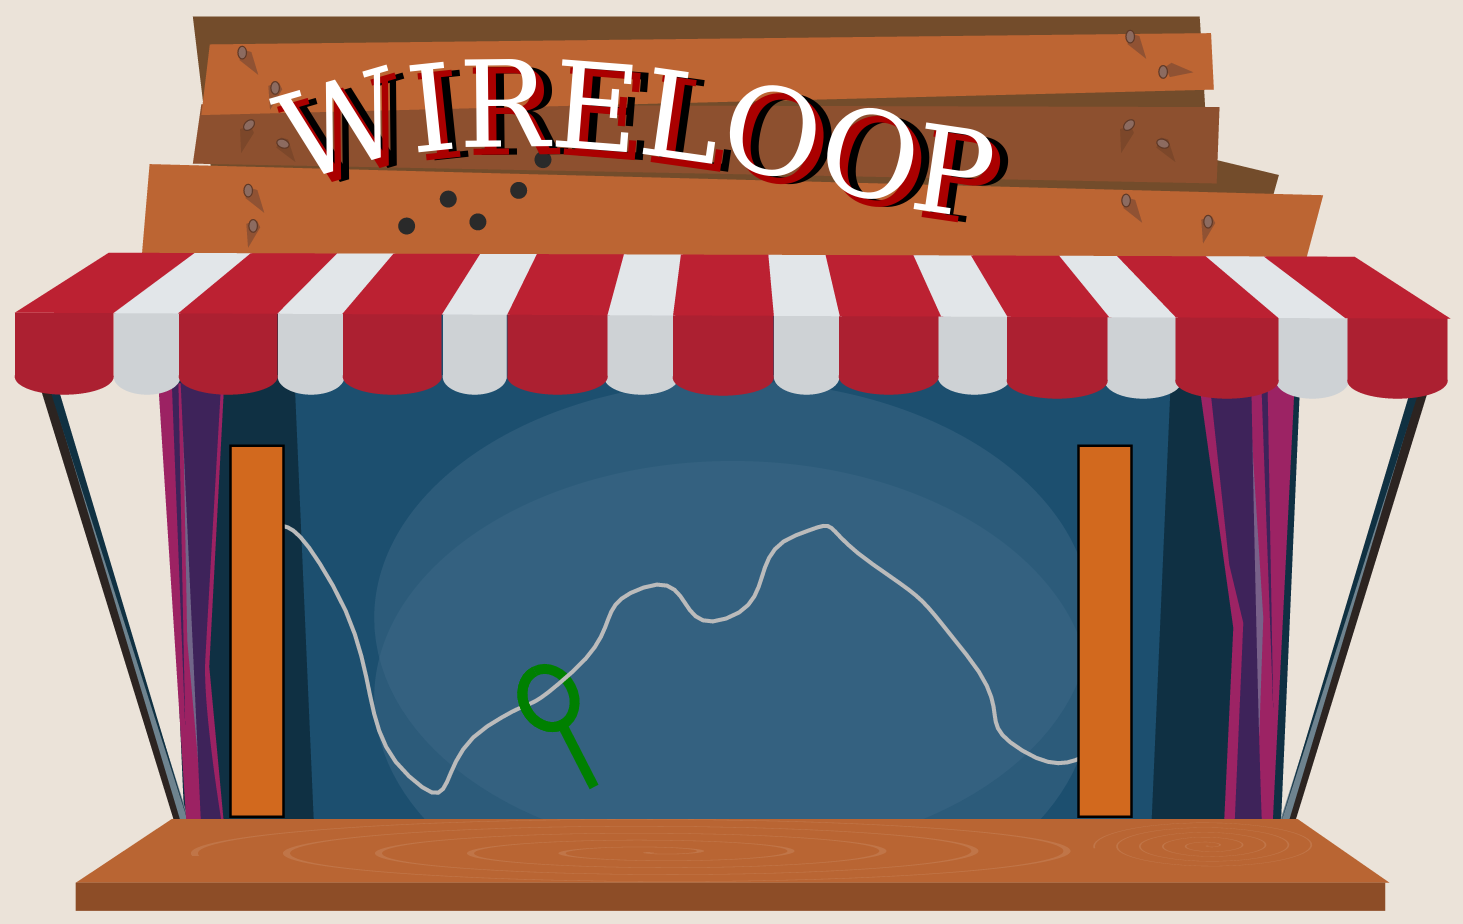
\includegraphics[width=0.25\textwidth]{images/wireloop.png}}\hfill
	\subfloat[Mastermind]{\label{ex5}
		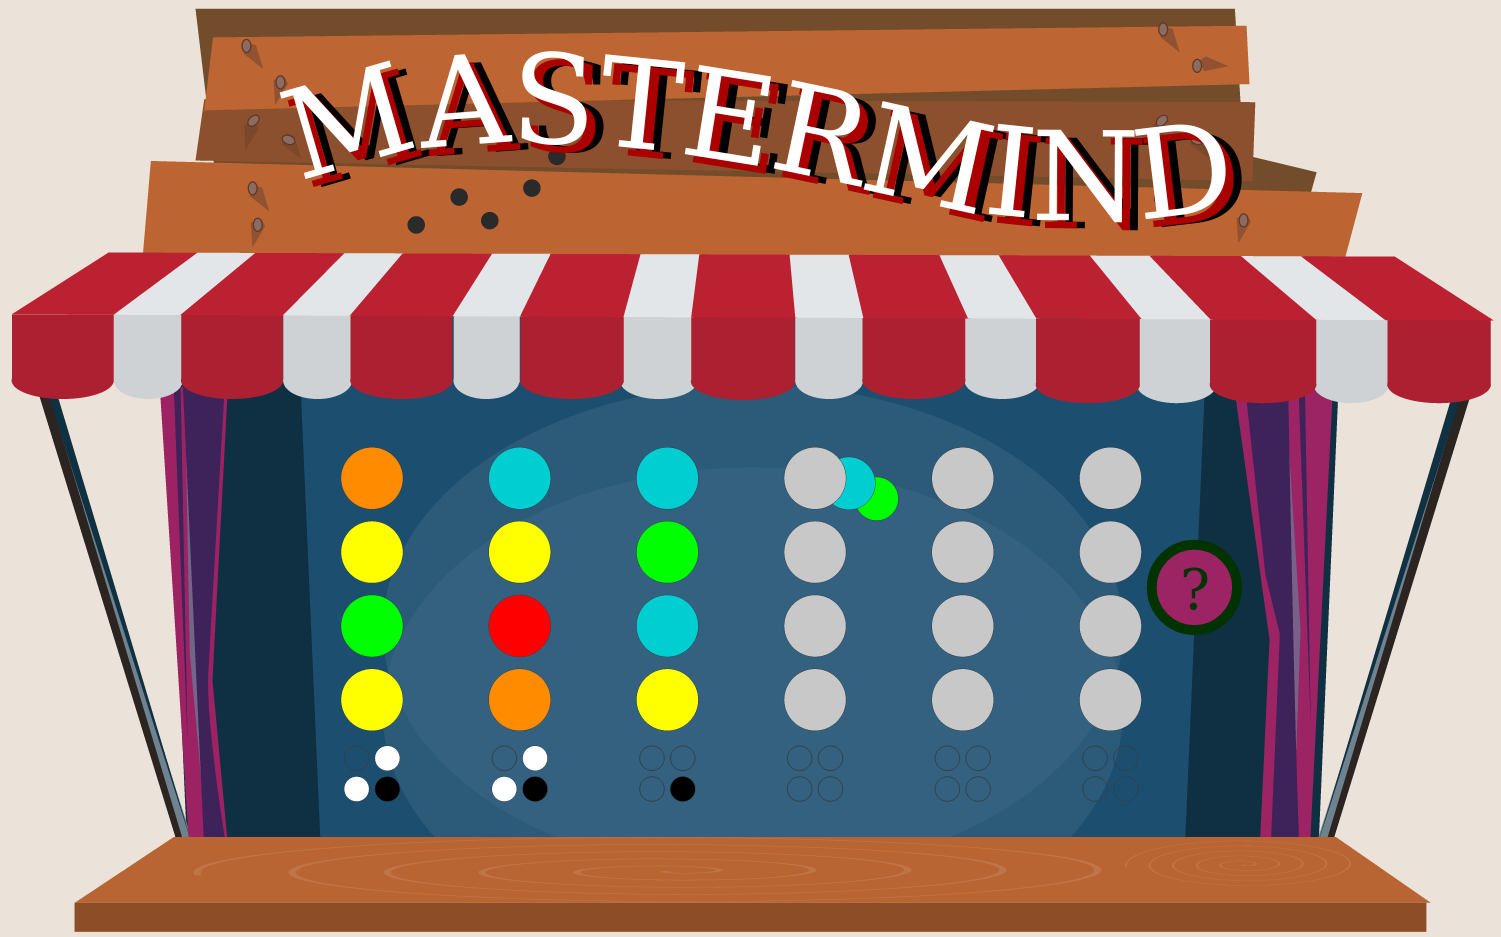
\includegraphics[width=0.25\textwidth]{images/mastermind.png}}\hfill
	\subfloat[Balancing]{\label{ex6}
		
\includegraphics[width=0.25\textwidth]{images/balancing.png}}
	\caption{Screenshots of all six browser games.}
\end{figure*}

\subsection{Mastermind}
Mastermind is a board game where one player selects a four-digit, order-sensitive color code and the other player tries to infer this code based on the feedback he receives in several rounds of guessing: Basically, for every token in the correct position (i.e. matching the code's color at this position), one receives a black feedback token; for every correctly colored token (that is, the color appears in the code) in the wrong position, one receives a white feedback token. This game serves as a demonstration that also games with four different control events can be controlled with the Emotiv device. The full list of game commands (in brackets: corresponding mental commands) is: change row (\texttt{nod}), change column (\texttt{shake head}), change color (\texttt{clench teeth}) and finally do nothing (every other mental state / action). In our experience, it is quite interesting to play this game with head movements and mental commands for the first time, however after a while, one would like to use a less cumbersome mouse instead. As this was not the case for other games, we think this might point to the fact that using an EEG device to replace a mouse is a bit boring - after all, we are pretty good in controlling computers with mouse and keyboard on a daily basis, whereas games that can only be played with such a device seem to be way more interesting.


\subsection{Wireloop}
Wireloop is a remake of the classic children's game in which a metal loop has to be dragged from one end to the other, without touching a wire. Typically a loud sound is played when the wire is touched accidentally. In our funfair setting, the wireloop game is controlled by the gyroscope: By moving the head, the rotational change is translated into planar co-ordinates that enable the metal loop to move. The wire itself is generated randomly using cardinal splines and is fully parametrized. The game is restarted whenever the wire was touched. The angle of the loop is automatically adapted to the current position by taking the derivative of the current line segment.

The wireloop game demonstrates that the gyroscope of an Emotiv Insight device can be sufficient to play an interesting game, one that would allegedly be quite boring with a mouse but is a real challenge with head movement control. The wireloop's control mechanism could be used to build a more complex game where the loop itself is at a fixed x-position on the screen, whereas the wire itself moves from left to right (an adaption of the \texttt{flappy bird} game). Beyond that, one could use it in a simulation game - e.g. for an aircraft cockpit where tilting the head would correspond to the plane tilting to a side.

\subsection{Balancing}
Our balancing game is perhaps the most challenging game, as it requires to balance a little man on an inherently instable seesaw: if tilted to one side, one needs to strain oneself in order to get it back to balance - but then, it tilts to the other side and one instantly needs to switch to 'zen mode', to total relaxation... if one is able to do this for 30 seconds, the game is won, otherwise it is re-started.

In some relaxation techniques such as \textit{Progressive Relaxation} \cite{Jacobson1938}, being able to consciously change from straining oneself to relaxation mode (and vice versa) is a core element: if one learns and trains how to change between these states, this can be effortlessly applied in situations where one is naturally stressed and tense, such as ahead of an exam or a job interview. It would be interesting to explore whether a game like our balancing game could be used in a similar fashion - which would then enable one to teach relaxation techniques to a broader variety of people than those attracted by, say, evening classes.

\begin{figure*}[h!]
	\centering
	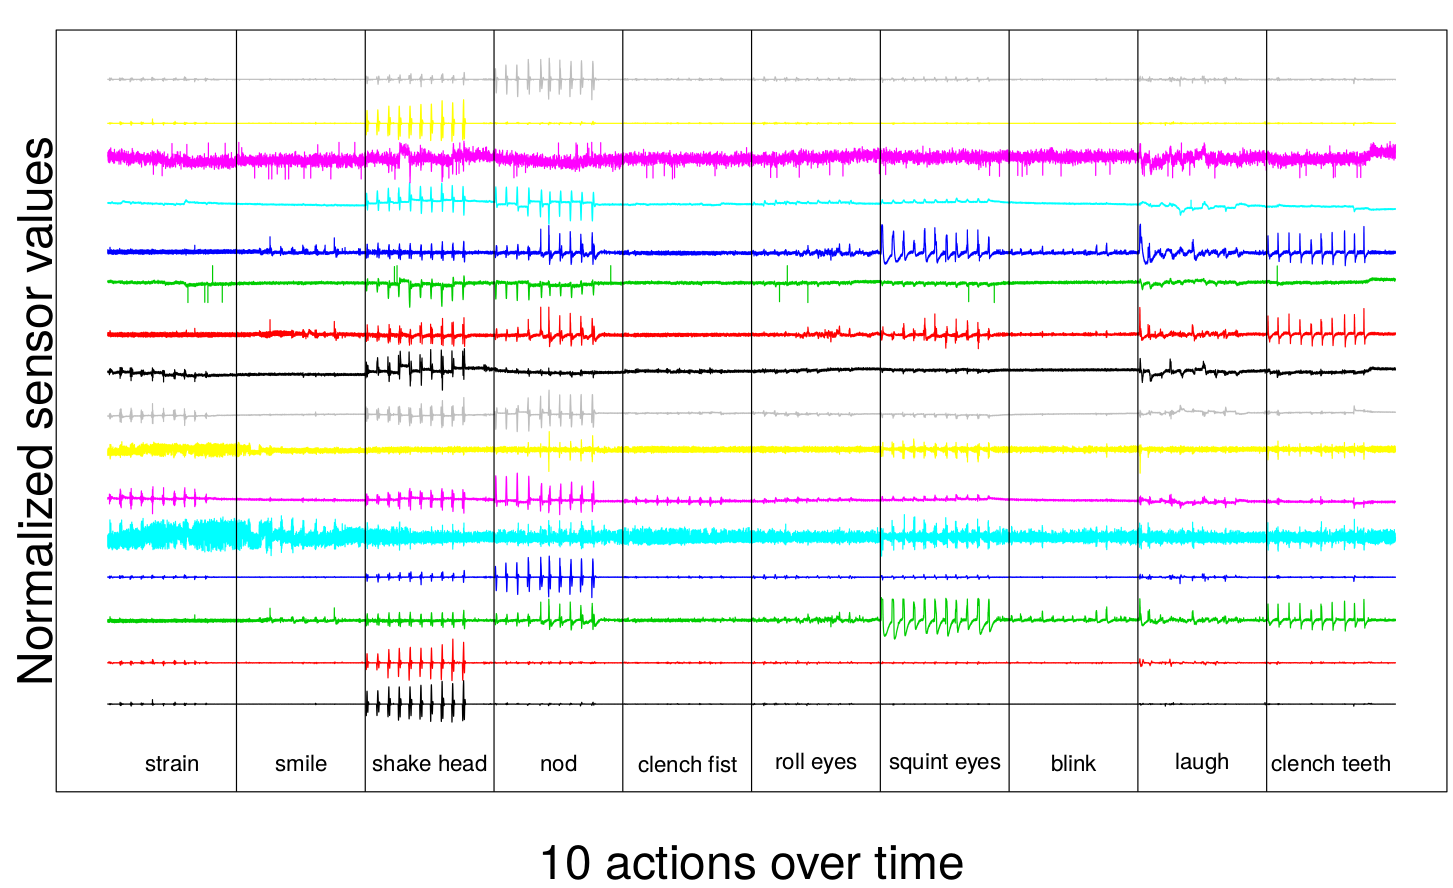
\includegraphics[width=1.0\textwidth]{images/sensor_values.png}
	\caption{Raw sensor data for ten different actions and mental commands. All data are normalized to lie within [0, 1]. Every sensor has a different offset here for better visibility. Sensors from top to bottom: \texttt{Y, X, F4, FC6, AF4, F8, T8, P8, O2, O1, P7, T7, F7, AF3, FC5, F3}. Every action corresponds to one minute of data recording, during which over the first 45 seconds the action was briefly executed every five seconds, followed by a short break until the next type of action began.}
	\label{fig:sensor_values}
\end{figure*}

\section{Possible Extensions}

Beyond the possible game-specific extensions and applications mentioned beforehand (highstriker: ADHD treatment through learning how to calm down, wireloop / gyroscope: flappy bird adaption with moving wire or aircraft simulation game, balancing: teach relaxation techniques), we could think of a couple of ways to enhance our funfair. It would be possible to add additional games without much effort, as the whole funfair is designed in a modular way. Beyond that, one could improve the visual experience of all our games by making them look more realistic, such as by using more sophisticated game engine or a 3D framework.

We anticipate our main contribution, however, to lie in an extensive exploration of different mouse- and keyboard-free game control mechanisms and the demonstration which forms of game control work well from a technical and data-driven perspective as well as from a user-centered point of view. Our work could be a starting point for future game designers implementing their own, unique ideas while being informed by our experiments on what forms of control serve a new, interesting gaming experience.

\bibliographystyle{alpha}
\bibliography{bibliography}

\end{document}

